\documentclass[10pt]{exam}

\usepackage[margin=1in]{geometry}
\usepackage{amsmath}
\usepackage{amssymb}
\usepackage{amsthm}
\usepackage{mathtools}
\usepackage{bm}
\usepackage{stmaryrd}
\usepackage{etoolbox}

\usepackage{color}
\usepackage{colortbl}
\definecolor{deepblue}{rgb}{0,0,0.5}
\definecolor{deepred}{rgb}{0.6,0,0}
\definecolor{deepgreen}{rgb}{0,0.5,0}
\definecolor{gray}{rgb}{0.7,0.7,0.7}

\usepackage{hyperref}
\hypersetup{
  colorlinks   = true, %Colours links instead of ugly boxes
  urlcolor     = black, %Colour for external hyperlinks
  linkcolor    = blue, %Colour of internal links
  citecolor    = blue  %Colour of citations
}

%%%%%%%%%%%%%%%%%%%%%%%%%%%%%%%%%%%%%%%%%%%%%%%%%%%%%%%%%%%%%%%%%%%%%%%%%%%%%%%%

\theoremstyle{definition}
\newtheorem{problem}{Problem}
\newtheorem{defn}{Definition}
\newtheorem{note}{Note}
\newtheorem{refr}{References}
\newtheorem{theorem}{Theorem}
\newcommand{\E}{\mathbb E}
\newcommand{\R}{\mathbb R}
\DeclareMathOperator{\nnz}{nnz}
\DeclareMathOperator{\determinant}{det}
\DeclareMathOperator{\Var}{Var}
\DeclareMathOperator{\rank}{rank}
\DeclareMathOperator{\prob}{\mathbb P}
\DeclareMathOperator*{\argmin}{arg\,min}
\DeclareMathOperator*{\argmax}{arg\,max}

\newcommand{\Ein}{E_{\text{in}}}
\newcommand{\Eout}{E_{\text{out}}}
\newcommand{\Etest}{E_{\text{test}}}
\newcommand{\Ntest}{N_{\text{test}}}
\newcommand{\I}{\mathbf I}
\newcommand{\Q}{\mathbf Q}
\newcommand{\p}{\mathbf P}
\newcommand{\pb}{\bar {\p}}
\newcommand{\pbb}{\bar {\pb}}
\newcommand{\pr}{\bm \pi}

\newcommand{\trans}[1]{{#1}^{T}}
\newcommand{\loss}{\ell}
\newcommand{\w}{\mathbf w}
\newcommand{\wstar}{{\w}^{*}}
\newcommand{\x}{\mathbf x}
\newcommand{\y}{\mathbf y}
\newcommand{\lone}[1]{{\lVert {#1} \rVert}_1}
\newcommand{\ltwo}[1]{{\lVert {#1} \rVert}_2}
\newcommand{\lp}[1]{{\lVert {#1} \rVert}_p}
\newcommand{\linf}[1]{{\lVert {#1} \rVert}_\infty}
\newcommand{\lF}[1]{{\lVert {#1} \rVert}_F}

\newcommand{\ignore}[1]{}

%%%%%%%%%%%%%%%%%%%%%%%%%%%%%%%%%%%%%%%%%%%%%%%%%%%%%%%%%%%%%%%%%%%%%%%%%%%%%%%%

\begin{document}


\begin{center}
{
\Huge
Chapter 1: The Learning Problem (II)
}
\end{center}

\begin{center}
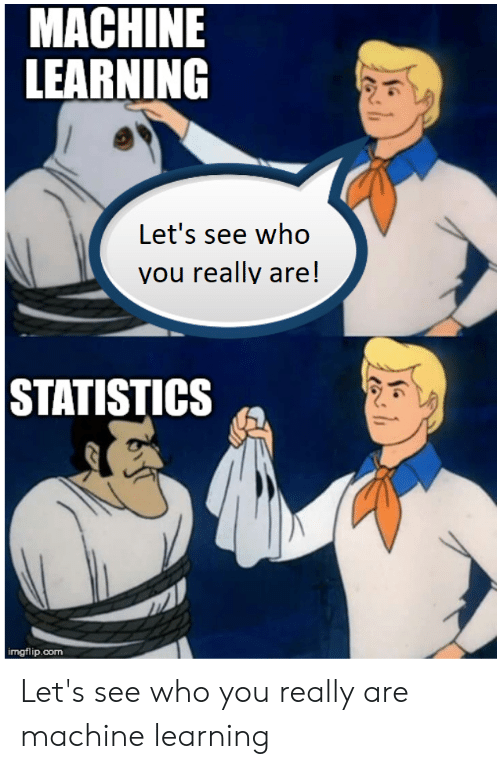
\includegraphics[height=3in]{scooby}
~~~~~~~~~~
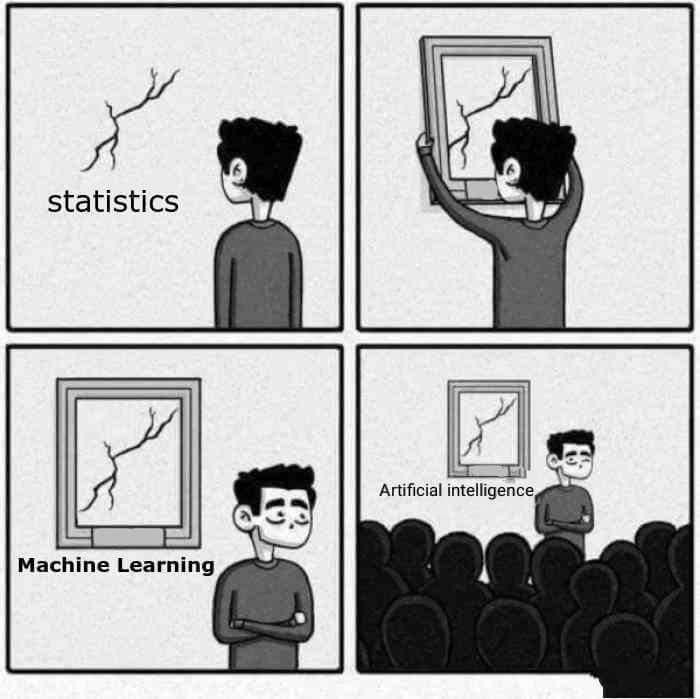
\includegraphics[height=3in]{ml}
\end{center}

%\section*{Section 1.1.3: Learning vs Design}
%
%\begin{problem}
%You should complete Exercise 1.5 to get practice identifying when to use a learning approach to a problem, and when to use a ``design'' approach to a problem.
%\end{problem}

%\section*{Section 1.2: Types of Learning}
%
%\begin{note}
%The textbook identifies 3 types of learning: supervised, reinforcement, and unsupervised.
%Pagerank is an example of an unsupervised algorithm (because we do not have ``labels'' about which nodes in the graph are the most important).
%The focus of most of this class will be on supervised methods.
%\end{note}

%\begin{problem}
    %You need to be able to identify examples of the different learning types.
    %Exercise 1.6 will give you practice with this.
%\end{problem}

%\newpage
\section*{Section 1.3: Is Learning Feasible? and \\ Section 1.4: Error and Noise and \\
Section 2.2.3 The Test Set}

%\begin{note}
    %The first note packet had you draw Figure 1.2.
    The previous note packet focused on the \emph{computational} component of learning.
    We used the Perceptron Learning Algorithm (PLA) as an example and derived its runtime.

    This packet introduces the \emph{statistical} component of learning.
    We will start by exploring the idea of training and testing sets,
    and see why they are used to evaluate model performance.
    Later notes will explore many other statistical components of learning.
    %They introduce the needed terms to understand whether an algorithm gives a ``good result'' independent of how long it took to get that result.

    It is very easy to get the computational and statistical aspects of learning confused.
    You should pay careful attention to the differences, which are highlighted in Figure 1.2, 1.9, and 1.11.
%\end{note}
%\begin{problem}
    %Draw Figure 1.11, highlighting the differences between Figure 1.9 and Figure 1.2.
%\end{problem}

%\begin{problem}
    %When our dataset , it is impossible to ``guarantee'' that we get the correct solution when training.
    %Read Section 1.3.1 and complete Exercise 1.7 to see an example problem 
%\end{problem}

%\newpage
%\begin{problem}
    %We say a binary learning problem is \emph{realizable} if it is possible to to get a perfect any of the following equivalent statements are true:
    %\begin{enumerate}
        %\item There is no noise in the targets.
            %That is, $P(y | \x) = f(\x)$.
        %\item
            %The best possible testing error is 0.
            %That is
            %$$
            %\argmin_{h\in\mathcal H} \Eout(h) = 0.
            %$$
    %\end{enumerate}
    %The runtime analysis we completed for the 
%\end{problem}

\newpage
\begin{problem}
    The PLA fails to converge (i.e.\ has an infinite runtime) if the input data is not linearly separable.
    Describe two scenarios that cause the PLA to fail to converge.
\end{problem}
\vspace{4in}

\begin{problem}
    %In this problem we will explore the train/test split protocol for training machine learning algorithms.
        Define the in-sample error (page 21), out-of-sample error (page 21), true/bayes error, and generalization error (page 40).
        %\item 
\end{problem}

\vspace{4in}

\newpage
\begin{note}
A fundamental goal of the machine learning discipline is to understand the out-of-sample error.
One of the most powerful tools for doing this is Hoeffding's inequality.
It is introduced informally in the textbook on page 19, Eq (1.4) in the context of a toy example involving marbles.
The following theorem is a formally stated version of this inequality,
and what you should rely on in this class.
\end{note}
\begin{theorem}[Hoeffding Inequality]
    Let $a_1, ..., a_N$ be $N$ independent and identically distributed random variables satisfying $0 \le a_i \le 1$.
    Let $\nu = \tfrac1n\sum_{i=1}^N a_i$ be the empirical average and $\mu = \E \nu$ be the true mean of the underlying distribution.
    Then, for all $\epsilon > 0$,
    \begin{equation}
        \label{eq:hoef}
        %\prob\big(|S_n - \E[S_n]| \ge t\big)
        \prob\big(|\nu - \mu| \ge \epsilon\big)
        \le 
        2 \exp (-2\epsilon^2 N)
        .
    \end{equation}
\end{theorem}
\begin{problem}
Describe the shape of the distribution defined by inequality \ref{eq:hoef} above.
\end{problem}

        \newpage
        %\item Let $g$ be the output of running the PLA on the training data.
            %What does Hoeffding's inequality say about the out-of-sample error?
            %\vspace{6in}

    %\end{enumerate}
%\end{problem}
%\newpage
%\begin{problem}
    %How large of a test set do you need to guarantee with probability at least 0.99 that $|\Etest-\Eout| \le 0.01$?
%\end{problem}

\newpage
\begin{problem}
    It is common to divide our data points into a \emph{training set} and a \emph{test set}.
    Recall that we let $N$ denote the size of the training set, $(\x_1, y_1),...,(\x_N,y_N)$ denote the training data points, and $\Ein$ the error on the training set.
    Similarly, we let $\Ntest$ denote the size of the test set,
    $(\x^{\text{test}}_1, y^{\text{test}}_1), ..., (\x^{\text{test}}_{\Ntest}, y^{\text{test}}_{\Ntest})$ denote the test data points, and
    $$
    \Etest(h) 
    =
    \
    \frac1{\Ntest} \sum_{i=1}^{\Ntest} \llbracket h(\x_i) \ne y_i \rrbracket
    $$
    denote the error on the test set.

    Now let $g$ be the result of running some learning algorithm on the training dataset.
    (The algorithm could be the PLA,
    or it could be some other algorithm that we haven't covered yet.)
    We would like to know $\Eout(g)$,
    since this is the true performance of the hypothesis $g$ on future data.
    We cannot calculate this quantity directly,
    but we can calculate $\Etest(g)$ and use the Hoeffding inequality to bound $|\Eout(g) - \Etest(g)|$.
    We want this quantity to be small.
    The subproblems below explore how big the test set must be in order to ensure that $\Eout$ is close to $\Etest$.
    %A common way of estimating the out of sample error $\Eout(g)$ is to use a \emph{test set}.
    %Let $\Ntest$ be the size of a ``test set'' that is used to evaluate a hypothesis
    %This problem explores how to use Hoeffding's inequality to to determine the size of your test set.
    %The initial 4 parts work with concrete numbers,
    %and part 5 i
    %The trend identified in the last portion is important to ``memorize''.
    \begin{enumerate}
        \item If you have a test set with 1000 samples, what bound does the Hoeffding inequality give on the probability that $|\Etest-\Eout| < 0.01$?

            HINT: Let $\Etest=\nu$ and $\Eout=\mu$.  Then recall that $P(|\Etest - \Eout) \ge \epsilon) = 1 - P(|\Etest - \Eout| < \epsilon)$.

            ANSWER: -0.637
            \vspace{2.5in}


        \item
            Why is this bound ``trivial''?

            ANSWER:
            The bound above says that the probability is greater than a negative number.
            This is always true by definition because a probability is between 0 and 1.
            When a bound doesn't provide any new information,
            we call it \emph{trivial}.
            \vspace{3.5in}

        \item
            What if you change the accuracy to $|\Etest-\Eout| \le 0.05$?

            ANSWER: 0.987
            \vspace{3.5in}

        \item
            What if you use the original accuracy $|\Etest-\Eout| \le 0.01$ but use 10000 samples in your test set?

            ANSWER: 0.729
            \vspace{3.5in}

    \end{enumerate}
\end{problem}

%\begin{problem}
    %MNIST is a famous dataset for optical character recognition.
    %Given an input picture, the goal is to predict what letter the image represents.
    %This is an example of a non-binary classification problem (or multiclass classification problem) because the output set $\mathcal Y = \{0, 1, 2, 3, 4, 5, 6, 7, 8, 9\}$.
%
    %The MNIST dataset has 70000 data points.
    %These points have been randomly split into 60000 training points and 10000 test points.
%
    %Three standard datasets for image classification are MNIST, CIFAR10, and ImageNet.
%
    %\begin{tabular}{lrr}
        %Dataset & training set size & test set size \\
        %\hline
        %MNIST & 60000 & 10000 \\
        %CIFAR10 & 50000 & 10000 \\
        %ImageNet & 60000 & 10000 \\
    %\end{tabular}
%\end{problem}

\newpage
\begin{note}
    The calculations in the previous problem are all examples of how a statistician would apply Hoeffding's inequality.
    In particular, the properties of the learning problem ($N$, $\Ntest$) was fixed,
    and we computed confidence intervals based on the given data.
    These computations are closely related to $p$-values and statistical testing.

    That is not how data miners operate.
    In the real world, problems are not statically given to us like they were in the problem above.
    Problems can be changed in order to make them easier to solve, and
    data miners use tools like Hoeffding's inequality to guide these changes.
    The following problem illustrates this concept.
    It is derived from a real capstone project.
\end{note}
\begin{problem}
            You are a consultant for BigBank.
            BigBank has trained a model $g_\text{house}$ for predicting whether to give a house loan to a client,
            and another model $g_\text{car}$ for predicting whether to give a car loan to client.
            Experiments show that
            \begin{align*}
                \Etest(g_\text{house}) &= 0.05 \\
                \Etest(g_\text{car}) &= 0.30
            \end{align*}
            Unfortunately, the test sets for both problems are rather small, with only 100 data points each.
            You have been given an additional budget to collect data to expand one of these test sets to 10000 data points,
            but unfortunately budget constraints will only let you enlarge one test set and the other will remain small.
            Which test set should you enlarge and why?
\end{problem}

\ignore{
\begin{problem}
    The goal of PAC learning bounds is to help us choose which model to use for a particular problem.
    (Recall that a model is a hypothesis class plus a learning algorithm.)
    In this problem, we will explore some simple, finite hypothesis classes.
\end{problem}

\begin{theorem}[Union Bound]
    For any set of events $\mathcal B_1, ..., \mathcal B_n$,
    we have that
    \begin{equation}
        \prob\left(\bigcup_{i=1}^n \mathcal B_i\right)
        \le
        \sum_{i=1}^n \prob(\mathcal B_i)
        .
    \end{equation}
\end{theorem}

%\begin{problem}
    %Define the
    %\begin{enumerate}
        %%\item Hoeffding Inequality (page 19, Eq 1.4)
        %%\item in-sample error (page 21)
        %%\item out-of-sample error (page 21)
        %\item Eq 1.5
        %\item union bound (page 24)
        %\item Eq 1.6
    %\end{enumerate}
%\end{problem}

\begin{problem}
    In practice, computers implement IEEE754 floating point arrithmetic rather than real number arithematic.
    This means that all hypothesis classes (that are used in practice) are actually finite.
\end{problem}

\begin{problem}
    Complete Exercise 1.11.
\end{problem}

\begin{problem}
    Complete Exercise 1.12.
\end{problem}

%\section*{Section 1.4: Error and Noise}
%
\begin{problem}
    Complete Exercise 1.13
\end{problem}

\begin{problem}
    For each statement below, indicate whether the claim is True, False, or Open.
    \begin{enumerate}
        \item More complicated models need a larger training set to deterime
    \end{enumerate}
\end{problem}

}

\newpage
\begin{problem}
Let $g$ be the output of running the PLA on a dataset of size $N$.
It is tempting to
let $\nu = \Ein(g)$ and $\mu=\Eout(g)$,
and then apply the Hoeffding inequality to state that the generalization error 
%$
    %|\Ein(g) - \Eout(g)|
%$
is bounded with high probability by
$$
    \prob(|\Ein(g) - \Eout(g)| \ge \epsilon) \le 2 \exp(-2\epsilon^2 N).
$$
Why is this not correct?

HINT: What assumption does Hoeffding require that we satisfied in the previous problem bounding $|\Etest - \Eout|$, but we do not satisfy in this problem bounding $|\Ein - \Eout|$?
\end{problem}
\end{document}



